\newpage

\chapter{\textsc{Огляд технології FHE}}


\section{Оначення}
В цій секції описана термінологія, яка використовується в дослідженнях FHE. Деякі з 
визначень були взяті напряму з документів FHE, інші були перефразовані для того, щоб
спростити формальність і зробити їх більш застосованими до обраної задачі.

Нехай є простір вхідного (чистого) тексту \(\mathcal{P}=\{0,1\}\), та сімейства функцій
\(F={f_1,f_2,...,f_n}\) де \(f_n(x) = f(x_1,x_2,x_3,...,x_k)\) це Булеві функції k
аргументів: \(f: P^n \rightarrow P\). Ми будемо називати F, сімейством Булевих схем
(Boolean circuit) \(C\), і використовувати звичайний запис функції \(C(m_1,m_2,...,m_n)\),
для позначення оцінки Булевої схеми на кортежі \((m_1,m_2,...,m_n)\).

\begin{definition}[\(\mathcal{C}\)-схема розрахунків, або ж просто \(\mathcal{C}\)-схема \cite{cryptoeprint:2011/344}] 
    Нехай \(\mathcal{C}\) це множина Булевих схем, тоді \(\mathcal{C}\)-схема розрахунків, для
    \(\mathcal{C}\) це набір функцій \((\textsc{gen, enc, eval, dec})\) які задовільняють наступним твердженням:


\(\textsc{\textbf{gen}}(1^\lambda,\alpha)\) - алгоритм генерації ключів, на вхід він приймає,
параметр шифрування \(\lambda\), та допоміжний параметр \(\alpha\). Результат виконання
алгоритму це триплет ключів \((pk,sk,evk)\), де ключ \(pk\) використовується для шифрування,
\(sk\) для дешифрування, та  \(evk\) для виконування розрахунків.

\(\textsc{\textbf{enc}}(pk,m)\) - алгоритм шифрування, на вхід він приймає ключ шифрування \(pk\) та
фрагмент не зашифрованого (чистого) тексту \(m\). Результат виконання алгоритму це шифр \(c\).

\(\textsc{\textbf{eval}}(evk,C,c_1,c_2...,c_n)\) - алгоритм розрахунків. На вхід він отримує,
ключ розрахунків \(evl\) та Булеву схему \(C \in \mathcal{C}\), та вхідні аргументи, які
можуть бути як шифром, так і результатом виконання минулих розрахунків. Результат виконання
алгоритму це результат виконання розрахунків.

\(\textsc{\textbf{dec}}(sk, c)\) - алгоритм дешифрування. На вхід приймає, ключ дешифрування
\(sk\), та шифр, або результат виконання розрахунків. Результат виконання алгоритму це не
зашифрований (чистий) текст \(m\).
\end{definition}

Для подальшого опису властивостей, треба визначити простори даних, які є результатами, або
вхідними параметрами описаних алгоритмів:

Нехай \(\mathcal{X}\) буде описувати простір \emph{чистого шифру}, \(\mathcal{Y}\) -
простір результатів виконання розрахунків, і \(\mathcal{Z} = \mathcal{X} \cup \mathcal{Y}\).
\(\mathcal{Z^*}\) - містить кортежі довільної довжини, які складаються
з елементів \(\mathcal{Z}\). Простори ключів згенерованих \textsc{\textbf{gen}},
позначимо як \(\mathcal{K}_p,\mathcal{K}_s,\mathcal{K}_e\) для \(pk,sk,evk\) відповідно.Алгоритм \textsc{\textbf{gen}} приймає на вхід параметр в унарній нотації \(1^\lambda\)
та опціональний допоміжний параметр \(\lambda\) з простору \(\mathcal{A}\). Також,
\(\mathcal{C}\) містить простір \emph{дозволених} булевих схем, а \(\mathcal{P}\), як було
зазначено раніше, область вхідного \emph{чистого (незашифрованого)тексту}.

Тепер можна описати область роботи наведених вище алгоритмів:
\begin{center}
    \begin{tabular}{l}
        \textsc{\textbf{gen }}: 
        \begin{math}
            \mathbb{N}\ \times\ \mathcal{A}\ \rightarrow\ 
            \mathcal{K}_p\ \times\ \mathcal{K}_s\ \times \ \mathcal{K}_e
        \end{math}\\

        \textsc{\textbf{enc }}:
        \begin{math}
            \mathcal{K}_p\ \times\ \mathcal{P}\ \rightarrow\ \mathcal{X}
        \end{math}\\

        \textsc{\textbf{eval}}:
        \begin{math}
            \mathcal{K}_e\ \times\ \mathcal{C}\ \times\ \mathcal{Z}^*\ 
            \rightarrow\ \mathcal{Y}
        \end{math}\\

        \textsc{\textbf{dec }}:
        \begin{math}
            \mathcal{K}_s\ \times\ \mathcal{Z}\ \rightarrow\ \mathcal{P}
        \end{math}
    \end{tabular}
\end{center}

Тоді \(\mathcal{X}\) та \(\mathcal{Y}\) можна визначити наступним чином:
\begin{center}
    \begin{math}
        \mathcal{X}\ =\ \{c\ |\ \textsc{\textbf{enc}}(pk,m)\ =\ c,\ m\ \in\ \mathcal{P}\}
    \end{math}
    \begin{math}
        \mathcal{Y}\ =\ \{z\ |\ \textsc{\textbf{eval}}(evk,C,c_1,c_2,...,c_n) = z,\ c_i\ \in\ 
        \mathcal{Z},\ C\ \in\ \mathcal{C} \}
    \end{math}
\end{center}
В деяких схемах, ключі розрахунків та шифрування однакові, але часто це і не так, тому в
визначеннях було наведено більш спільний випадок.

В оригінальних документах FHE \cite{cryptoeprint:2011/344} не було зазначено, що алгоритм
розшифровування \textsc{\textbf{dec}} повинен мати можливість працювати з результатом виконання
алгоритму шифрування \textsc{\textbf{enc}} - \(\mathcal{X}\), і було зазначено, що данні
можуть бути розшифровані після виконання розрахунків над ними \textsc{\textbf{eval}} - 
\(\mathcal{Y}\). Для можливості розшифровування, зразу після зашифровування було запропоновано
мати \emph{чисту Булеву схему} або ж по суті функцію \(f(x)=x\), для виконання розрахунків і
отримання даних які вже можна буде розшифровувати. Більшість сучасних FHE схем, дозволяють
проводити операції дешифрування даних, над якими не було проведено розрахунків, тому я не буду
заглиблюватись в цю тему.

\subsection{Атрибути та властивості}
Тут представлені характеристики методів гомоморфного шифрування. Ми встановлюємо такі
властивості, як компактність і конфіденційність схеми, які забороняють спрощені рішення
задачі гомоморфного шифрування, з одного боку, і вимагають таких властивостей, як
коректність, для того, щоб навіть називати це схемою шифрування.

\begin{definition}[Коректне розшифровування \cite{cryptoeprint:2015/1192}]
\label{def:corr-dec}
\(\mathcal{C}\)-схама має атрибут коректного розшифрування якщо виконується наступне твердження:
\begin{center}    
    \begin{math}
        \textsc{\textbf{dec}}(sk,\textsc{\textbf{enc}}(pk,m)) = m
    \end{math},\\
    де \(pk,sk,evk \leftarrow \textsc{\textbf{gen}}(1^\lambda,\alpha)\), \(\alpha \in \mathcal{A}\), \(m \in \mathcal{P}\).
\end{center}
Це означає, що ми повинні мати можливість безпомилково розшифровувати зашифрований текст.
\end{definition}

\begin{definition}[Коректні розрахунки \cite{cryptoeprint:2015/1192}]
\label{def:corr-eval}
\(\mathcal{C}\)-схема коректно розраховує всі Булеві схеми \(C \in \mathcal{C}\), якщо
виконується наступне твердження:
    \begin{center}
        \begin{math}
        \textsc{\textbf{dec}}(sk,\textsc{\textbf{eval}}(evk,C,c_1,c_2,...,c_n))\ 
        =\ C(m_1,m_2,...m_n)
        \end{math},\\
        \(pk,sk,evk \leftarrow \textsc{\textbf{gen}}(1^\lambda,\alpha)\), \(\alpha \in \mathcal{A}\), \(c_i \in \mathcal{X}\) та \(m_i \leftarrow \textsc{\textbf{dec}}(sk,c_i)\)
    \end{center}
Це визначення означає, що розрахунки над зашифрованими даними з подальшим
розшифровуванням повинні бути однакові з результатом розрахунків над не зашифрованими
даними.
\end{definition}

Будемо називати \(\mathcal{C}\)-схему \emph{коректною} якщо для неї будуть виконуватись
(Озн. \ref{def:corr-dec}) та (Озн. \ref{def:corr-eval}) твердження.

\begin{definition}[Компактність \(\mathcal{C}\)-схеми]
\label{def:compactness}
    \(\mathcal{C}\)-схема вважається компактною якщо існує поліном \(p\), такий що, для
    будь-якого кортежу \((pk,sk,evk) \leftarrow \textsc{\textbf{gen}}(1^\lambda,\alpha)\), \(\alpha \in \mathcal{A}\), будь-якої Булевої схеми \(C \in \mathcal{C}\) та
    шифру \(c_i \in \mathcal{X}\), розмір результату виконання
    \(\textsc{\textbf{eval}}(evk,C,c_1,c_2,...,c_n)\) не більше від \(p(\lambda)\)
    бітів, в не залежності від Булевої схеми.
\end{definition}
Озн.чення \ref{def:compactness}, показує що під час гомоморфних операцій розмір
результату не повинен збільшуватись, і залежить тільки від параметра безпеки \(\lambda\).

\begin{definition}[Компактно розрахункова \(\mathcal{C}\)-схема \cite{homenc}]
\label{def:compactl-eval}
\(\mathcal{C}\)-схема компактно розраховує всі Булеві схема \(C \in \mathcal{C}\), якщо
вона компактна (Озн. \ref{def:compactness}) та \emph{коректна}.
\end{definition}

\subsubsection*{Безпека схеми}
Далі, важливо зупинитись на безпеці та конфіденційності схеми. Безпеку схеми можна
розділити на дві компоненти: семантична безпека, та обфускація схеми. Якщо обфускація
використовується коли алгоритм шифрування секретний, і вразливий, то семантична безпека
описує розподіл вихідних даних з \textsc{\textbf{eval}} та \textsc{\textbf{enc}}.
\begin{definition}[Конфіденційне гомоморфне шифрування схеми \cite{homenc}(2.16)]
\label{def:conf-eval}
    \(\mathcal{C}\)-схема вважається безпечною, якщо для будь-якого кортежу \((pk,sk,evk) \leftarrow \textsc{\textbf{gen}}(1^\lambda,\alpha)\), \(\alpha \in \mathcal{A}\), будь-якої Булевої схеми \(C \in \mathcal{C}\) та
    шифру \(c_i \in \mathcal{X}\), такого що \(m_i \leftarrow \textsc{\textbf{dec}}(sk, c_i)\) існує два розподіли:

\begin{center}
    \begin{math}
        Dist_1 = \textsc{\textbf{eval}}(evk,C,c_1,c_2,...,c_n)
    \end{math}\\
    \begin{math}
        Dist_2 = \textsc{\textbf{enc}}(pk,C(c_1,c_2,...,c_n)
    \end{math}
\end{center}
які повинні бути статистично або обчислювально нерозрізнені. Ці вимоги показують,
що розподіл виконання обчислень Булевої схеми над шифром \(Dist_1\) повинен бути однаковий (статистично, обчислювально) з розподілом, отриманим шляхом зашифровування
\emph{чистого} тексту, який насамперед являється результатом виконання Булевої операції 
над незашифрованими даними \(Dist_2\).

Часто термін безпечної системи можна зустріти як \emph{Сильно гомоморфна система}\cite{Clear_2013}. 
\end{definition}

\subsection{Класифікація}
Оскільки не всі схеми FHE мають однакові властивості, цей розділ показує як схеми
класифікуються, в залежності від того, які схеми вони можуть обчислювати.

\begin{definition}[Частково Гомоморфна схема або \(\mathcal{C}\)-Гомоморфізм \cite{cryptoeprint:2011/344}]
\label{def:part-he}
\(\mathcal{C}\)-схема називається, частково гомоморфною (SHE), якщо вона має коректне
шифрування (Озн. \ref{def:corr-dec}), та коректне обчислення (Озн. \ref{def:corr-eval}). 
\end{definition}
Для частково гомоморфних \(\mathcal{C}\)-схем нема вимог до компактності, тому з кожним
гомоморфним розрахунком розмір вихідного шифру може збільшуватись. Також нема ніяких
вимог до множини Булевих операцій які можуть бути використовувані для розрахунків.

\begin{figure}[!ht]
    \centering
    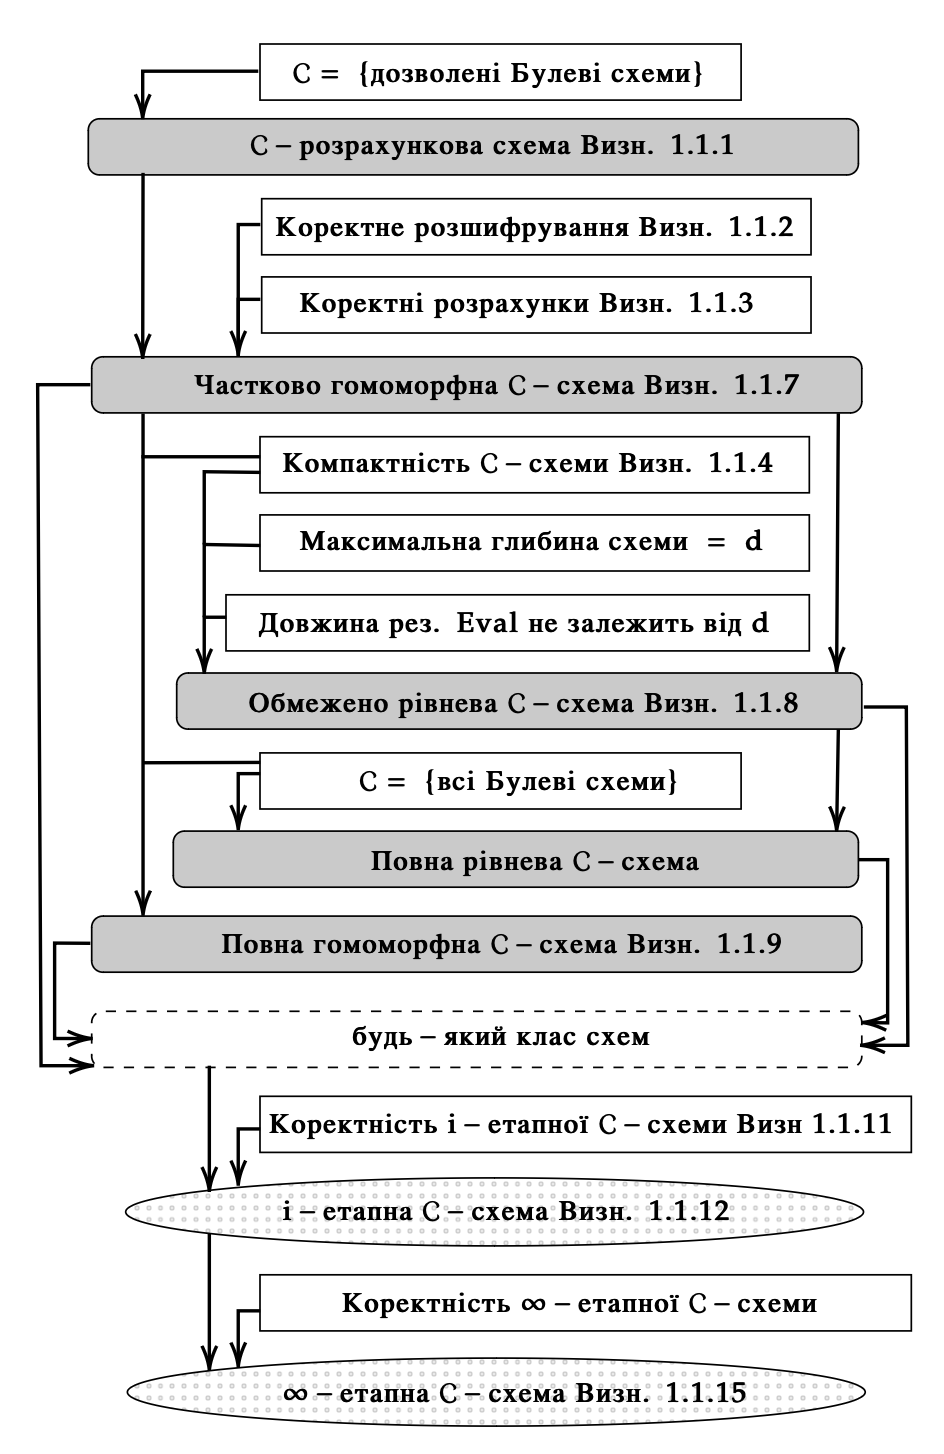
\includegraphics[scale=0.75]{static/classification.png}
    \caption{Дерево класифікацій \(\mathcal{C}\)-схем. Прямокутниками позначені визначення,
    закруглені затемнені прямокутники, позначають класи \(\mathcal{C}\)-схеми, а еліпси
    позначають розширення для етапних розрахунків. Стрілки показуть залежність одного 
    твердження від іншого.}
    \label{fig:classification}
\end{figure}

\begin{definition}[Обмежено-рівнева Гомоморфна схема]
\(\mathcal{C}\)-схема називається Обмежено-рівневою, якщо алгоритм генерації ключів
\textsc{\textbf{gen}} приймає додатковий параметр \(\alpha=d\), який означає максимальну
глибину Булевої схеми, яка може бути обчислена. Також застосовані вимоги до компактності,
коректності, і те що розмір вихідних даних розрахунків не повинен залежати від d.

\end{definition}

\begin{definition}[Повна Гомоморфна схема]
\label{def:fhe}
Повною гомоморфною схемою, називають \(\mathcal{C}\)-схему, до якої застосовані вимоги,
коректності, компактності, та вона може обчислювати Булеву схему з множини усіх схем, або
ж будь-яку схему.
\end{definition}

\subsection{Композиція розрахунків}
Часто, задача потребує декілька послідовних розрахунків, тобто результат певної Булевої
схеми повинен слугувати вхідними даними для наступної схеми, або ж простими словами
можна це назвати - композиція.
Кожну операцію розрахунків над шифром \textsc{\textbf{eval}} будемо називати \emph{етапом розрахунків}. 

З визначення коректних розрахунків \ref{def:corr-eval} видно що вхідні дані для
алгоритму обчислення \textsc{\textbf{eval}} повинні належати множині \(\mathcal{X}\) -
або ж множині \emph{чистого шифру}, який є результатом алгоритму \textsc{\textbf{enc}}.
Цей розділ описує вимоги, виконуючи які алгоритм розрахунку схеми \textsc{\textbf{eval}},
може приймати на вхід як результат виконання інших розрахунків \(\mathcal{Z}\), так і
\emph{чистий шифр} \(\mathcal{X}\): 

\(\textsc{\textbf{eval}}(evk, C, c_1,c_2,...,c_n)\),
де \((pk,sk,evk) \leftarrow \textsc{\textbf{gen}}(1^\lambda,\alpha)\), \(\alpha \in \mathcal{A}\), \(C \in \mathcal{C}\) та \(c_i \in \mathcal{X} \cup \mathcal{Z}\)

В літературі \emph{розрахунки з етапами} називають \textbf{\emph{гомоморфним шифруванням
з i-етапами}}(i-hop homomorphic encryption \cite{10.1007/978-3-642-19571-6_14},
\cite{cryptoeprint:2010/145})

\begin{definition}[Розрахунки з етапами]
\label{def:stage-eval} 
    Обчислення \(\textbf{C}_{i,n}\) в \(i\) етапів, та шириною \(n\), визначається множиною
    Булевих схем \(\{C_{kl}\}\), де \(1 \leq k \leq i,1 \leq l \leq
    \) n, та \(C_{kl}\) має \(kn\) вхідних даних. За вхідними даними \(m_{01},m_{02},...,m_{0n}\) ми
    обчислюємо:
\begin{center}
    \(m_{kl} = C_{kl}(m_{01},m_{02},...,m_{0n},...,m_{k-1,1},...,m_{k-1,n})\), де \(1 \leq k \leq i,1 \leq l \leq n\).
\end{center}
Результат розрахунків з етапом після \textsc{\textbf{eval}} та \textsc{\textbf{dec}} буде 
\emph{чистий текст} \(m_{i1},m_{i2},...,m_{in}\). Озн.чимо початковий \emph{чистий текст} як
\(\overrightarrow{m_0}\), та вихідний \emph{чистий текст} як \(\overrightarrow{m_i}\), тоді можна
записати співвідношення \(\overrightarrow{m_i} = C_{i,n}(\overrightarrow{m_0})\).


Нехай \((pk,sk,evk) \leftarrow \textsc{\textbf{gen}}(1^\lambda,\alpha)\), \(\alpha \in \mathcal{A}\),
та \(c_{i1},c_{i2},...,c_{in} \in \mathcal{X}\), тоді шифр \(\{c_{kl}\}\), 
\(1 \leq k \leq i,1 \leq l \leq n\) обчислюється рекурсивно наступним чином:
\begin{center}
    \(c_{kl} = \textsc{\textbf{eval}}(evk,C_{kl},c_{01},...,c_{0n},...,c_{k-1,1},...,c_{k-1,n})\)
\end{center}
Результат розрахунків з етапом над зашифрованими даними, буде шифр \(c_{i1},c_{i2},...,c_{in}\).
Позначивши початковий (вхідний) шифр як \(\overrightarrow{c_0}\) та результівний шифр як 
\(\overrightarrow{c_i}\) можна описати співвідношення яке описує нотацію алгоритму \textsc{\textbf{eval}}
з декількома виходами: \(\overrightarrow{c_i} = \textsc{\textbf{eval}}(evk,C_{1,n},\overrightarrow{c_0})\)
\end{definition}

\begin{figure}[ht!]
    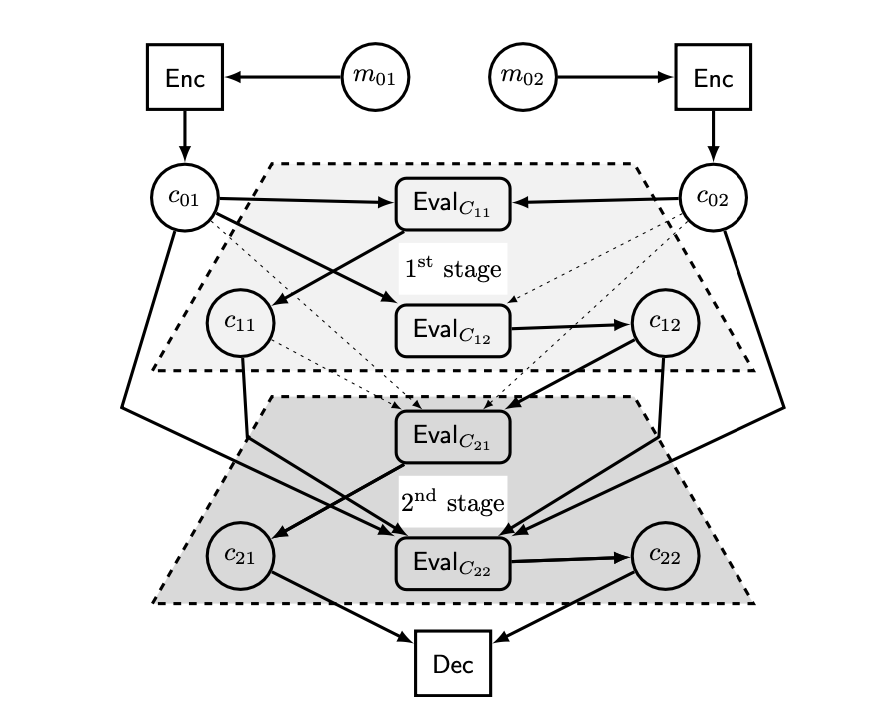
\includegraphics[]{static/I-hop-eval.png}
    \caption{Приклад \cite{cryptoeprint:2015/1192} гомоморфного шифрування з i-етапами,
    де \(i=2,n=2\)}
    \label{fig:i-hop-eval}
\end{figure}

З вище описаного визначення \ref{def:stage-eval} можна зробити висновок що вхідними даними для
будь-якого етапу, окрім першого, може бути \textsc{тільки} результат попереднього етапу.

На перший погляд, може здатись, що якщо у нас є можливість обчислити довільну Булеву схему, не
використовуючи \(i\)-етапне шифрування, то повинна бути можливість обчислювати багато схем
послідовно. Проте це не так. Нема гарантій того, що результат виконання \textsc{\textbf{eval}},
буде валідний для використання як вхідні дані для наступного \textsc{\textbf{eval}}.
Наведемо приклад \cite{cryptoeprint:2015/1192}: Нехай у нас є схема \(C\) яка приймає на вхід
\(c_1,c_0,...,c_n\), та результатом якої є \(c'_0,c'_1,...,c'_v\), та схема \(C'\), яка приймає
на вхід \(c_0,c_1,...,c_v\) та результат якої \(c'_0,c'_1,...,c'_w\). Тоді існує 2 можливих 
сценарії: 1) Якщо ми візьмемо композицію \(C\) та \(C'\) як схему для розрахунків
\textsc{\textbf{eval}}(evk, \(C \circ C'\), \(c_1,c_2,...,c_n\)) то ці розрахунки будуть
коректними, оскільки виконується одна Булева схема, 2) проте, якщо ми спочатку розрахуємо
\textsc{\textbf{eval}}(evk, \(C\), \(c_1,c_2,...,c_n\)) = \(c'_1,c'_2,...,c'_v\), а потім
\textsc{\textbf{eval}}(evk, \(C'\), \(c'_1,c'_2,...,c'_v\)) то це не спрацює зі звичайною
схемою повного гомоморфного шифрування, оскільки вона не гарантує коректність даних після
розрахунків, для наступних операцій. Тому якщо стоїть задача виконання послідовних, незалежних
обчислень, то варто використовувати схему з i-етапами.

\begin{definition}[Коректність гомоморфного шифрування з i-етапами]
\label{def:i-hop-eval-corr}
Нехай \((pk,sk,evk) \leftarrow \textsc{\textbf{gen}}(1^\lambda,\alpha)\), \(\alpha \in \mathcal{A}\),
та \(\textbf{C}_{i,n}=\{C_{k,l}\}\) - довільне поетапне обчислення, де \(n\) це розмір
полінома від \(\lambda\) та \(\overrightarrow{c_0}=(c_{01},c_{02},...,c_{0n}) \in
\mathcal{X}^n\). Тоді \(\mathcal{C}\)-схему можна вважати коректною з і-етапами, якщо
виконується наступне твердження:
\begin{center}
    \begin{math}
        \textsc{\textbf{dec}}(sk,\textsc{\textbf{eval}}(evk,\textbf{C}_{i,n},
        \overrightarrow{c_0})) = \textbf{C}_{i,n}(\textsc{\textbf{dec}}(sk,\overrightarrow{c_0}))
    \end{math}
\end{center}
\end{definition}
Хоча це визначення і дуже схоже на визначення коректності розрахунків \ref{def:corr-eval},
проте важливо розуміти, що наведене вище визначення застосоване до розрахунків з
багатьма етапами, про що свідчить \(\textbf{C}_{i,n}\) = \(\{C_{k,l}\}\).


На Рис. \ref{fig:i-hop-eval} зображений приклад розрахунків з етапами, де \(i=2,n=2\).

Тепер, маючи загальне визначення коректності гомоморфного шифрування, можна описати більш
часткові випадки шифрування з i-етапами, а саме: i-етапне, мульті-етапне, полі-етапне та
\(\infty\)-етапне.

\begin{definition}[i-етапна \(\mathcal{C}\)-схема \cite{cryptoeprint:2010/145}]
    \label{def:i-stages}
    Нехай \(i \in \mathbb{N}\), тоді \(\mathcal{C}\)-схема \(i\)-етапна, якщо вона
    коректна для всіх \(j\)-етапних схем, де \(1 \leq j \leq i\).
\end{definition}

Замість того щоб параметризувати етапи числом, як в визначенні i-етапної схеми: \(i \in 
\mathbb{N}\), етапи можуть залeжaти від полінома параметризовані \(\lambda\).

\begin{definition}[мульті-етапна \(\mathcal{C}\)-схема \cite{cryptoeprint:2010/145}]
    \label{def:multi-stages}
    Нехай \(p\) - деякий поліном, тоді \(\mathcal{C}\)-схема називається мульті-етапною,
якщо вона коректна для всіх \(j\)-етапних схем, таких  що: \(1 \leq j \leq p(\lambda)\).
\end{definition}

\begin{definition}[полі-етапна \(\mathcal{C}\)-схема \cite{cryptoeprint:2015/1192}]
    \label{def:poli-stages}
    Нехай \(p\) - деякий поліном, та \(\alpha \in \mathcal{A}\), тоді 
    \(\mathcal{C}\)-схема називається полі-етапною, якщо вона коректна для 
    всіх \(j\)-етапних схема, таких  що: \(1 \leq j \leq p(\lambda, \alpha)\).
\end{definition}

\begin{definition}[\(\infty\)-етапнa \(\mathcal{C}\)-схема]
    \label{def:inf-stages}
    \(\mathcal{C}\)-схема називається \(\infty\)-етапною, якщо вона коректна для всіх \(j\)-етапних схем для всіх j.
\end{definition}

\subsection{Наслідки та об'єднання визначень}
Тепер ми детально розглянемо наслідки визначень, наведених у попередньому розділі. Спочатку
ми повернемося до питання компактності та її двох, здавалося б, окремих визначень.

Існує різниця між визначенням компактності яке було запропоноване в роботі Gentry 
\cite{homenc}, та між визначенням \ref{def:compactness}, цей розділ узгоджує ці два
визначення.

Для більшості результатів вимагається, щоб допоміжний параметр генерації ключа \(\alpha\)
був поліноміально обмежений \(\lambda\), хоча для всіх реалізованих схем це і так, 
формальної гарантії цього нема, тому в далі описаних визначеннях це буде вимагатись явно.

\begin{definition}[Gentry-компактність \cite{homenc}]
    \(\mathcal{C}\)-розрахункова схема вважається компактною за Gentry, якщо існує
    поліном \(f\), такий що, для кожного значення параметра безпеки \(\lambda\), алгоритм
    дешифрування може бути виражений у вигляді Булевої схеми \(C_{Dec}\) розміром максимум
    \(f(\lambda)\).
\end{definition}

\begin{definition}[Gentry-компактно розрахункова схема \cite{homenc}]
\(\mathcal{C}\)-розрахункова схема вважається компактно разрахунковою за Gentry, якщо
для всіх Булевих схем \(C \in \mathcal{C}\) виконуються твердження коректності розрахунків
(Озн. \ref{def:corr-eval}), та коректності дешифрування (Озн. \ref{def:corr-dec}), та вона 
Gentry-компактна.
\end{definition}

Розмір Булевої схеми, це число логічних вентилів, або ж якщо представляти схему як граф, то
це число вершин.

На перший погляд не зрозуміло як два визначення компактності можуть бути узгоджені:
\begin{theorem}
    Нехай \(\lambda\) поліноміально обмежена \(\lambda\). \(\mathcal{C}\)-розрахункова
    схема Gentry-компактно розрахуновує \(\mathcal{C}\), тоді і тільки тоді, коли схема
    компактно обчислює \(\mathcal{C}\).
\end{theorem}
Доведення цієї теореми можна знайти в додатках до роботи Armknecht та інші. \cite{cryptoeprint:2015/1192}.

\begin{theorem}
    \label{theorem:ideal-conf-compactness}
    \(\mathcal{C}\)-розрахункова схема з ідеальною конфіденційністю схеми, передбачає
    компактність, коли \(\alpha\) поліноміально обмежена \(\alpha\).
\end{theorem}
Термін \emph{ідеальна конфіденційна схема} відноситься до визначення \ref{def:conf-eval} де
розподіл \(\mathcal{X}\) = \(\mathcal{Y}\), або ж абсолютно нерозрізнений.
Доведення цієї теореми можна знайти в додатках до роботи Armknecht та інші. \cite{cryptoeprint:2015/1192}.

\subsection{Зв'язок FHE та i-етапних схем}
Нехай \(\alpha\) поліноміально обмежена \(\lambda\), в цій секції будуть представлені
результати, що стосуються зв'язку FHE схем та i-стрибкових схем, припускаючи що \(\alpha\)
поліноміально обмежена \(\lambda\).

\begin{theorem}
    Повна гомоморфна (Озн. \ref{def:fhe}) \(\mathcal{C}\)-розрахункова схема, зі статистично конфіденційною
    схемою - мульті-етапна (Озн. \ref{def:multi-stages}).
\end{theorem}
Доведення теореми можна знайти в роботі Armknecht \cite{cryptoeprint:2015/1192}.

Тепер ми дослідимо зв'язок між повністю гомоморфною та i-етапою схемою, зазначивши, які
властивості повинна мати частково гомоморфна схема шифрування, щоб бути повністю
гомоморфною. По-перше, ми дослідимо, за яких умов повністю гомоморфна схема допускає
нескінченну кількість етапів обчислень:

\begin{theorem}
    \label{theorem:she-inf-hop}
    Частково гомоморфна (Озн. \ref{def:part-he}) \(\mathcal{C}\)-розрахункова схема з
    ідеальною конфіденційністю схеми - \(\infty\)-етапна (Озн. \ref{def:inf-stages}).
\end{theorem}

\emph{Доведення}: Оскільки схема має ідеальну конфіденційність (Озн. \ref{def:conf-eval}),
то розподіл результатів виконання \textsc{\textbf{eval}} ідентичний до розподілу виконання
схеми над \emph{чистим текстом}, або ж: \((\mathcal{X} = \mathcal{Y} = \mathcal{Z})\). Отже
результат виконання \textsc{\textbf{eval}} знову стає ваділдними вхідними даними, і не
залежить від того скільки разів були виконані розрахунки.

Теорема \ref{theorem:she-inf-hop} наводить на іншу теорему в оберненій формі:

\begin{theorem}
    Частково гомоморфна схема з Булевими схемами \(C \in \mathcal{C}\), які містять
    тільки NAND вентилі, ідеально конфіденційна та \(\infty\)-етапна (Озн. \ref{def:inf-stages}) - повна гомоморфна (Озн. \ref{def:fhe}).
\end{theorem}

\emph{Доведення}: Оскільки схема ідеально конфіденційна, то за Теоремою \ref{theorem:ideal-conf-compactness}, вона компактна, тоді для того щоб показати що вона повна комоморфна за
визначенням (Озн. \ref{def:fhe}) треба показати що вона може обчислювати будь-яку
булеву схему. Припустимо обернене, нехай існує Булева схема \(C\), яку схема не може
коректно обчислювати. Представимо що схема \(C\) складається лише з NAND вентилів.
Оскільки NAND \(\in C\) та схема \(\infty\)-етапна, ми можемо коректно обчислити
кожен NAND вентиль на відповідному вході, незалежно від того який рівень ітерації
обчислення має цей вхід. Таким чином, ми знайшли спосіб коректно розрахувати Булеву схему
використовуючи \(\mathcal{C}\)-схему, або ж \(C \in \mathcal{C}\), що суперечить припущенню
і показує що схема повністю гомоморфна.

Таким чином можна побудувати наступну діаграму, яка показує необхідні вимоги для 
виконання теореми, та її результат:

\begin{figure}[!h]
    \centering
    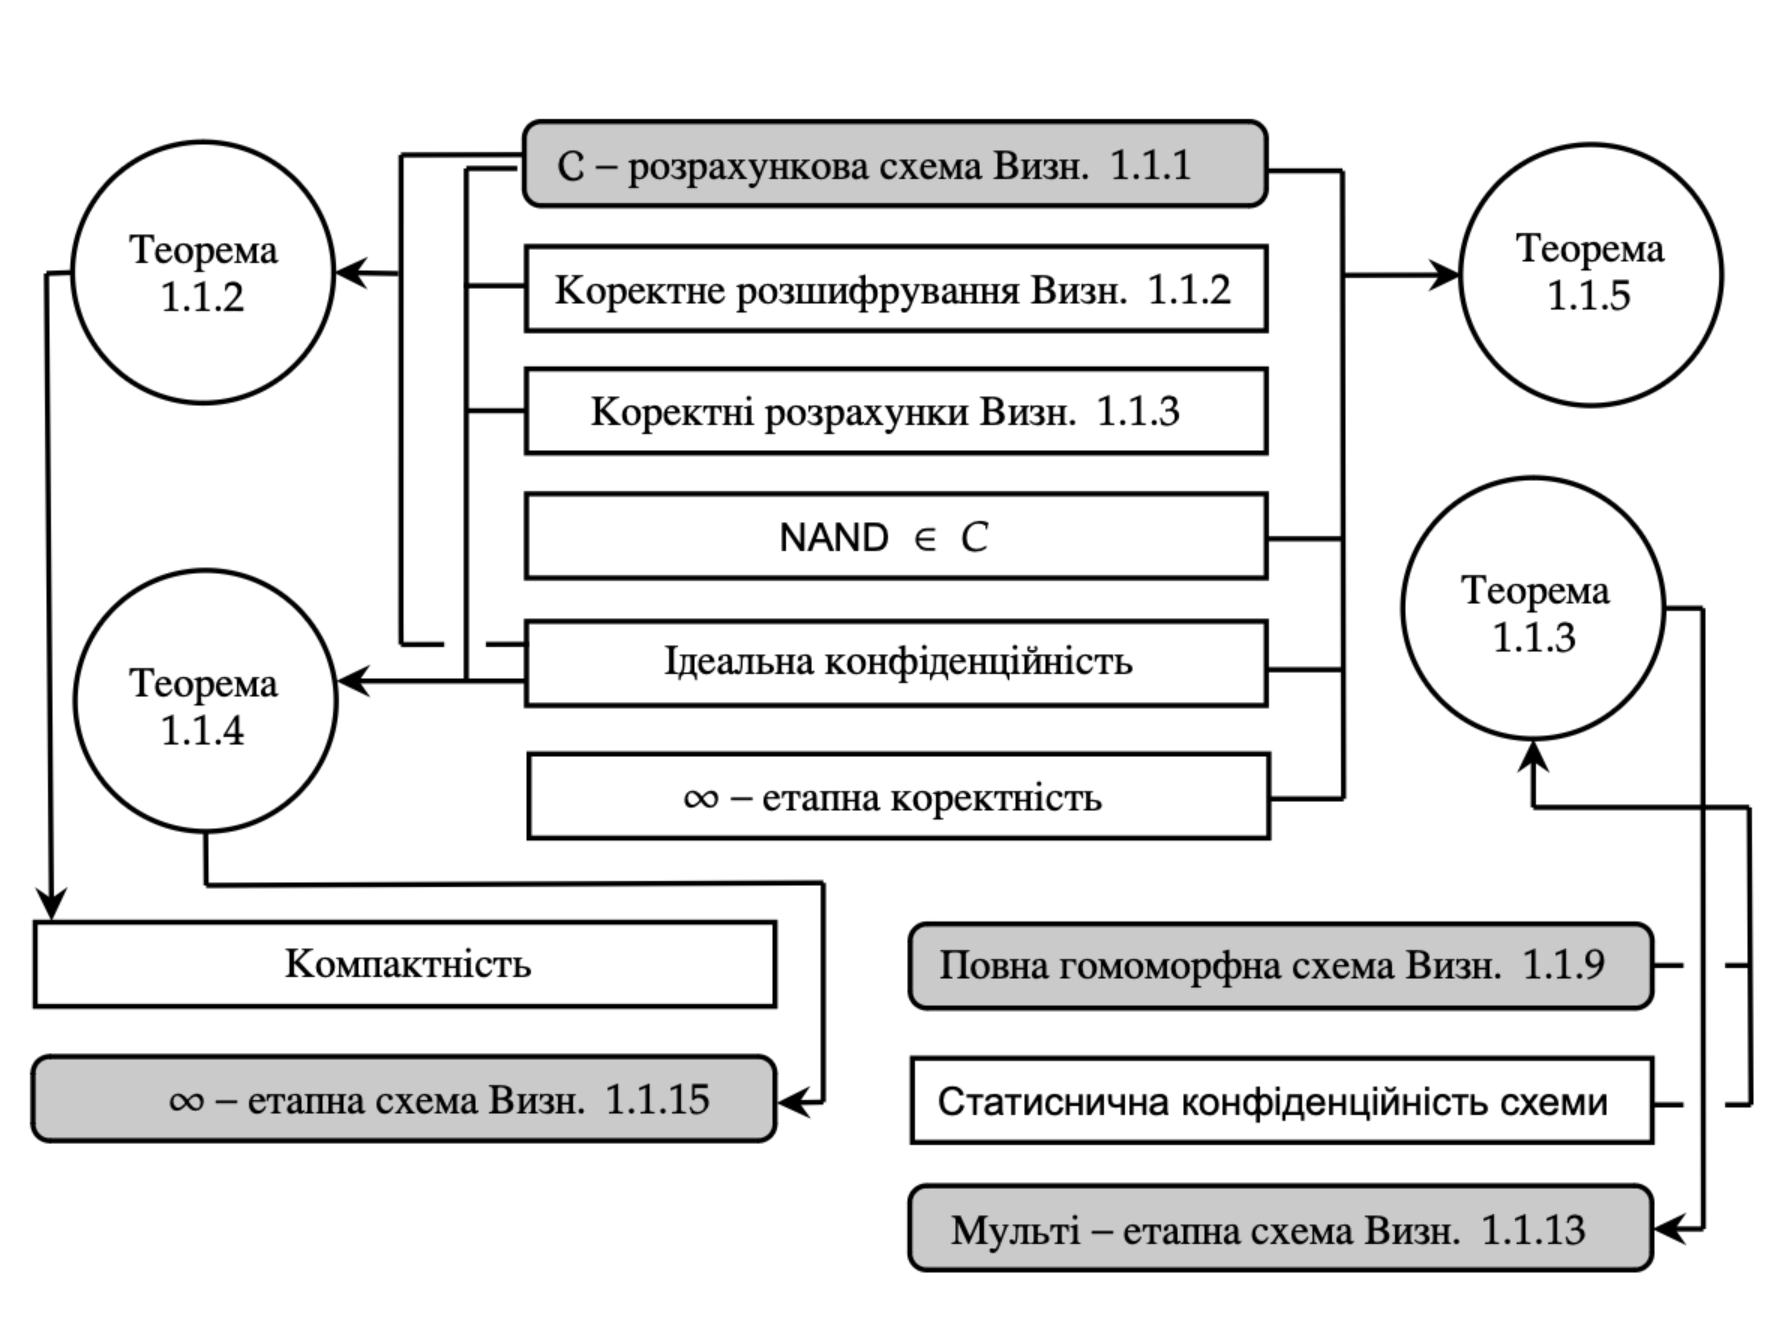
\includegraphics[scale=0.7]{static/fhe-i-hop-connection.png}
    \caption{Зв'язок необхідних вимог для теорем, та їх результатів}
    \label{fig:fhe-i-hop-connection}
\end{figure}

\section{Обмеження}
Існує велика кількість програм які використовують FHE для вирішування поставленої задачі. Проте
наразі існую обмеження у використання цієї технології, далі в цьому розділі буде розглянуто 
декілька з них. 

\begin{itemize}
    \item Перше обмеження FHE, це жорстка прив'язка пар ключів, що унеможливлює багатьом користувачам використовувати спільні дані. Уявимо ситуацію де багато
користувачів використовують систему яка, в свою чергу покладається на внутрішню базу 
даних для обчислень. Дані, які були додані в базу даних, можуть бути використані в
обчисленнях, тільки користувачем який їх туди додав. Тобто в ситуації коли багато 
користувачів повинні працювати над одними даними, щоб досягти спільної цілі - FHE 
обмежений. Проте існує гарний претендент на вирішення цього обмеження \cite{cryptoeprint:2013/094} Multikey Fully Homomorphic Encryption.

    \item Друге обмеження це те що FHE потребує дуже великих витрат на обчислення.
Розрахунки та проведення операцій над зашифрованими даними виконуються набагато довше ніж
на чистих незашифрованих даних. Хоча сучасні алгоритми FHE показують достойні 
покращення в часі на розрахунки, однак ця проблема все ще залишається одним із головних
аргументів не використовувати FHE. Запропоноване часткове розв'язання цієї проблеми, це 
використовувати Тьюрінг Машини замість Булевих схем \cite{10.1007/978-3-642-40084-1_30}.

    \item Третє обмеження полягає в тому що алгоритм розрахунків над зашифрованими,
даними не може бути зашифрований сам по собі. Тому, наприклад, маючи складний
алгоритм розрахунків акцій, який не повинен бути оприлюднений, складно використати в
контексті FHE. Часткове рішення цієї проблеми було запропоноване в роботі Michael 
Naehrig \cite{10.1145/2046660.2046682}, де він запропонував передавати функцію у зашифрованому вигляді.
Проте шифрування алгоритму це не зовсім область відповідальності FHE, і повинна
досягатись шляхом обфускації алгоритмів.

\end{itemize}

\section{Відомі області застосування}
В цьому розділі описані можливі області де може бути ефективно застосовані FHE. Будуть
описані як і повноцінні області де може бути застосована технологія, тек і використання
як допоміжного інструменту, для побудови більш комплексних систем.

\subsubsection*{Конфіденційність користувача у рекламних пропозиціях}
В сучасному світі реклама може бути не тільки набридливою для користувача, а напроти дуже
корисною, якщо алгоритми для підбору цієї реклами базуються на персональних даних,
користувача, таких як: його вподобання, рік народження, перегляд певних ресурсів та джерел,
локація  користувача тощо. Більшість людей відносяться до персональної безпеки дуже
відповідально, і не хочуть її розголошувати задля отримання персоналізованої реклами.

Для вирішення цієї проблеми чудово підходить FHE, оскільки він може виконувати алгоритми над
зашифрованими даними користувача.

В документі \cite{arjan2005} була описана одна з таких систем, де рекомендації для користувача
основані на рекомендаціях його друзів. Система застосовує гомоморфне шифрування, щоб була
можливість отримувати рекомендації друзів буз розголошення їх особистостей.

Інша реалізація задачі була описана в документі \cite{armfredthor2011}. В реалізації
користувач отримує рекомендації від системи, якій не важливо який контент їй був переданий, та
від якого користувача. Для побудови такого алгоритму, була зроблена проста, але дуже ефективна
FHE схема, яка дозволяє отримувати рекомендації для користувача, який залишається невидимим для
системи.

Ще одна робота, яка варта згадки \cite{10.1145/2046660.2046682}, забезпечує рекламні
рекомендації на базі локації користувача, виконуючи алгоритми над зашифрованими даними, що
не дозволяє зловмисникам отримати, де знаходиться користувач системи.

\subsubsection*{Конфіденційність даних пацієнта у медичних застосунках}

В роботі \cite{10.1145/2046660.2046682}, описане практичне використання FHE в медичних
застосунках, де важлива конфіденційність даних пацієнта. В описаній системі пацієнт робить
запит до системи зі своїми даними в зашифрованій формі, оскільки користувач системи це
власник даних, то тільки він може їх розшифрувати. Застосунок який реалізує сервіс, в свою
чергу, може рахувати, чи отримувати з баз даних, інформацію, таку як: група крові, тиск, 
серцебиття, хвороби та інше. за зашифрованими даними, результат роботи сервісу, також буде
зашифровані дані.

В роботі \cite{cryptoeprint:2011/405} була реалізована подібна система, яка рахує вірогідність
серцевого нападу, основуючись на зашифрованих даних пацієнта.

\subsubsection*{Інтелектуальний аналіз даних}
Аналіз даних на великих обсягах інформації дає гарний результат, проте ціна цьому результату
приватність даних користувачів.

Була зроблена чудова робота \cite{zhiqiang2005} яка реалізує логіку зашифрованого аналізу
даних, без втрати точності, і забезпечує безпеку за допомогою FHE схеми.

\subsubsection*{Конфіденційність фінансових операцій}
Хоча як було описано в розділі про обмеження, FHE і не забезпечує шифрування самого алгоритму,
його можна використовувати в іншому сценарії:

Представимо, що існує дві компанії X та Y, у компанії X є приватні акції, а у компанії Y є
секретний алгоритм який рахує прогноз по динаміці змін акцій. Тоді компанії X достатньо 
застосувати FHE для своїх даних, що дозволить рахувати над ними алгоритм компанії Y, без
дешифрування.

\subsubsection*{Криміналістичне розпізнавання зображень}
В роботі \cite{bosch2014} була представлена ще одна чудова сфера застосування FHE. 
Поліція та інші правоохоронні органи використовують подібні інструменти для пошуку нелегальних
фотографій на жорстких дисках, у мережевих потоках даних та інших наборах даних. Поліція
використовує базу даних "поганих" хеш-значень зображень. Можливість того, що злочинці можуть
отримати доступ до цієї бази даних, перевірити, чи будуть їхні фотографії розпізнані, і, якщо
так, змінити їх, викликає серйозне занепокоєння.

Ця схема реалізує сценарій, коли база даних поліції зашифрована, але водночас законний
мережевий трафік компанії залишається приватним завдяки використанню дещо гомоморфної
стратегії шифрування, запропонованої в наступному документі 
\cite{10.1007/978-3-642-22792-9_29}. Компанія протиставляє хешований і зашифрований потік
фотографій зашифрованій базі даних поліції. Тимчасова змінна надається поліції через
заздалегідь визначений проміжок часу або поріг, при цьому постачальник послуг нічого не
дізнається про саму зашифровану базу даних.

\subsubsection*{Хмарні обчислення з захищеними даними}
Гомоморфне шифрування дозволяє використовувати хмарні ресурси для обробки даних, не
розкриваючи їх змісту. Користувач може зашифрувати дані та передати їх в хмару для
виконання обчислень. Хмарний провайдер, використовуючи FHE, може виконати різні операції
над зашифрованими даними, такі як пошук, фільтрація або обчислення агрегатних функцій, не
розкриваючи вмісту даних. Результати обчислень повертаються користувачу, який може
розшифрувати їх і отримати оброблені дані.

\subsubsection*{Туманні обчислення}
FHE може бути використана в туманних обчисленнях для забезпечення безпечного виконання
обчислень на краю мережі (edge computing). Це особливо важливо в сферах, де важливо
зберегти конфіденційність даних, наприклад, в медичних додатках, додатках Інтернету речей
(IoT) або системах безпеки.

\subsection*{Використання FHE як інструмент для більш комплексних криптосистем}

Далі наведені приклади, як FHE може бути використаний як інструмент, для створення більш
складних криптографічних інструментів, таких як: цифрові  підписи, MACs, доведень з нульовим
розголошенням, та інш.

\subsubsection*{Делегування розрахунків}
Делегування обчислень - це другий великий стовп хмарних обчислень, окрім делегування даних.
Користувач може захотіти делегувати обчислення функції f серверу. Однак сервер може бути
зловмисним або просто схильним до збоїв, тобто користувач може не довіряти результатам
обчислень. Користувач хоче мати доказ того, що обчислення було виконано правильно, і перевірка
цього доказу також повинна бути значно ефективнішою, ніж виконання обчислень користувачем.


Одним із прикладів делегування обчислень є автентифікатори повідомлень. Користувач, який
делегував обчислення для набору даних, може захотіти перевірити, що
результат є дійсно правильним. Тег має бути незалежним від розміру вихідного набору даних, і
його може перевірити лише власник приватного ключа. Одна з таких схем була запропонована в
роботі \cite{10.1007/978-3-642-42045-0_16}, яку можна розглядати як симетрично-ключову версію
повністю гомоморфних підписів.

\subsubsection*{Цифрові підписи}
В документі \cite{cryptoeprint:2014/897}, вперше була запропонована конструкція підпису, 
на базі рівнево-повної гомоморфної схеми. Схема може розраховувати довільні Булеві схеми з
максимальною глибиною \(d\) над підписаними даними і гомоморфно генерувати короткий підпис,
який може бути перевірений будь-ким за допомогою відкритого ключа перевірки. 

\subsubsection*{Багатопарне обчислення}

Багатосторонні обчислення вимагають взаємодії між учасниками. Робота 
\cite{cryptoeprint:2011/535} надає опис того, як частково гомоморфна схема може бути
використана для побудови автономного множення під час обчислень. Користувачі використовують
дещо гомоморфну схему на етапі попередньої обробки, але повертаються до набагато ефективніших
методів багатосторонніх обчислень на етапі обчислень. Користувач завантажує підписані дані x,
потім сервер виконує над ними деяку функцію \(g\), яка дає \(y = g(x)\). Крім того, сервер
публікує підпис \(\tau_{g,y}\) для перевірки обчислень.

Ця робота також вводить поняття гомоморфних функцій лазівки (HTDF), одного з будівельних
блоків для побудови підпису. Самі HTDF базуються на проблемі малого цілочисельного розв'язку (SIS).

\section{Існуючі FHE схеми}
В цьому розділі будуть поверхнево описані існуючі FHE схеми. Будемо вважати початковою
точкою розвитку гомоморфних схем, роботу Gentry \cite{homenc}, до цієї роботи не 
відбувалось значного впливу на розвиток технологій.

Деякі схеми, які не підпадають під визначення компактності не будуть представлені, тому що
вони малозначущі в сучасному світі, такими схемами можна назвати: Fellows та Koblitz
\cite{fellows1994}. Деякі схеми підпадають під визначення компактності, але обмежені по
операції, наприклад схема Bohen-Goh \cite{10.1007/978-3-540-30576-7_18}. Такі схеми не
будуть розглядатись оскільки вони не вважаються повними гомоморфними за визначенням \ref{def:fhe}.

\begin{itemize}
    \item{\textbf{Gentry FHE \cite{homenc}} } 
    \item{\textbf{FHE через цілі \cite{cryptoeprint:2009/616}} }
    \item{\textbf{Пакетне повністю гомоморфне шифрування над цілими числами \cite{eurocrypt-2013-25038}} }
    \item{\textbf{Ефективна форма FHE через LWE \cite{cryptoeprint:2011/344}} }
    \item{\textbf{Повністю гомоморфне шифрування над LWE-кільцями та захистом повідомлень,
        що залежать від ключа \cite{10.1007/978-3-642-22792-9_29}} } 
    \item{\textbf{Повністю гомоморфне шифрування без перезавантаження (Озн. \ref{def:bootstraping}) \cite{journals/eccc/BrakerskiGV11}} }
\end{itemize}

\subsection{Перезавантаження схеми та альтернативи}
Ключовими моментами в створенні FHE схем є техніка перезавантаження схеми, яка була
представлена Gentry \cite{homenc}. Схема представлена в його документі вважалась зашумленою,
тобто, \emph{чистий текст} був схований за шумом, який пізніше знімався операцією
розшифровування. Проте цей шум збільшувався з кожною операцією над зашифрованим текстом,
і коли цей шум досягав критичної точки, то розшифровування тексту унеможливлювалось.

Щоб вирішити цю проблему, в документі була представлена техніка \emph{перезашифровування},
логіка якої було зашифровування, вже зашифрованого тексту, а при дешифруванні, спочатку
знімається верхній шифр, поки тест не стане \emph{чистим}. Тобто, якщо алгоритм 
розрахунків, може впоратись з процесом дешифрування + \textsc{NAND} вентилем, можна
досягти прогресу в розрахунках схеми, які необхідні.

\begin{definition}[Схильна до перезавантаження \(\mathcal{C}\)-схема]
    \label{def:bootstraping}
    Якщо \(\mathcal{C}\)-схема, може гомоморфно обчислювати свою власну Булеву схему
    дешифрування, плюс ще одну операцію \textsc{NAND}, то її можна вважати схильну до
    перезавантаження.
\end{definition}

Основне питання яке виникає до вище наведеного визначення: Чи не порушує безпеку публікація
зашифрованого приватного ключа (необхідного для дешифрування) під його власним публічним
ключем?

Якщо ми припустимо, що безпечно публікувати шифрування секретного ключа під відповідним
йому відкритим ключем, ми досягнемо повністю гомоморфного шифрування і навіть i-рівневого.
Таке припущення називається циклічною безпекою. Однак, якщо циклічна безпека не працює,
то однією з можливостей є використання ланцюжка пар відкритий ключ/секретний ключ, де
секретний ключ завжди зашифрований під наступним відкритим ключем. Це дозволяє відповідним
дещо гомоморфним схемам стати гомоморфними за рівнем, де рівень залежить від кількості пар
ключів.

Альтернативний спосіб досягнення гомоморфного шифрування належить Brakerski
\cite{cryptoeprint:2011/344}. Проблема все ще полягає в тому, як керувати шумом, але цього
разу це досягається за рахунок зменшення модуля простору зашифрованого тексту разом із
шумом.

Параметр безпеки, який диктує, наскільки малим може бути модуль, дає обмеження на кількість
рівнів. Цей напрямок роботи призводить до нативних рівневих гомоморфних схем. Однак автори
зазвичай зазначають, що можна застосувати перезавантаження як оптимізацію, а також як засіб
для отримання повністю гомоморфної схеми i-рівнів, знову ж таки, припускаючи кругову
безпеку.
